\documentclass[tikz,border=3pt]{standalone}
\usetikzlibrary{arrows.meta,decorations.pathmorphing}
\begin{document}
\pgfmathsetseed{2718}
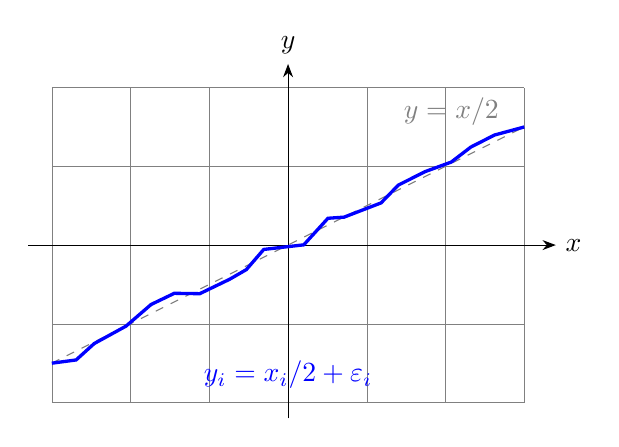
\begin{tikzpicture}[x=1cm,y=1cm,>=Stealth]
  \draw[help lines] (-3,-2) grid (3,2);
  \draw[->] (-3.3,0) -- (3.4,0) node[right] {$x$};
  \draw[->] (0,-2.2) -- (0,2.3) node[above] {$y$};
  \draw[gray,dashed] (-3,-1.5) -- (3,1.5);
  \draw[blue,very thick,decorate,
    decoration={random steps,segment length=3.5mm,amplitude=1.1mm}]
    (-3,-1.5) -- (3,1.5);
  \node[gray,above left] at (2.8,1.4) {$y=x/2$};
  \node[blue,below] at (0,-1.35) {$y_i=x_i/2+\varepsilon_i$};
\end{tikzpicture}
\end{document}
